\documentclass[color,twoside,amssymb,twocolumn]{article}
\usepackage{cite}
\usepackage{Latex-document}
\usepackage{bm}
\usepackage[usenames]{color}

\usepackage{times}
\usepackage{soul}
\usepackage{xcolor}
\usepackage{url}
\usepackage[hidelinks]{hyperref}
\usepackage[utf8]{inputenc}

%\usepackage[small]{caption}
%\usepackage{graphicx}
\usepackage{subfigure}
\usepackage{amsmath}
\usepackage{booktabs}
\usepackage{algorithm}
\usepackage{algorithmic}
\urlstyle{same}
\usepackage{float}
\usepackage{makecell}
\usepackage{amsthm,amsmath,amssymb}
\usepackage{mathrsfs}

\setlength{\paperwidth}{210truemm}
\setlength{\paperheight}{297truemm}

\definecolor{lightblue}{rgb}{0, 0, 0}
\renewcommand{\algorithmicrequire}{\textbf{Input:}}
\renewcommand{\algorithmicensure}{\textbf{Output:}}


%\definecolor{white}{rgb}{1,1,1}
%\definecolor{lightblue}{rgb}{0.052, 0.25, 1}



\setcounter{secnumdepth}{4}

\setcounter{subsection}{0}

%%%\bibliographystyle{unsrt}

%\newcommand{\titlename}{$\bm{Revenu}$-$\bm{Maximizing~ Online~ Stable~ Task~ Assignment~}$\\$\bm{on~ Taxi}$-$\bm{Dispatching~ Platforms}$\\[2mm]{\bf Instruction for authors}}
\newcommand{\titlename}{\bf Revenue-Maximizing Online Stable Task Assignment on Taxi-Dispatching Platforms}
\newcommand{\authorname}{Jingwei Lv$^{1}$ , Ze Zhao$^{2}$, Shuzhen Yao$^{1}$, Weifeng Lv$^{1}$}
\newcommand{\atime}{Received month 01.2021; accepted month 01.2021}
\newcommand{\aemail}{$lvjingwei@buaa.edu.cn$}

%\makeatletter
%\newenvironment{breakablealgorithm}
%{% \begin{breakablealgorithm}
%	\begin{center}
%		\refstepcounter{algorithm}% New algorithm
%		\hrule height.8pt depth0pt \kern2pt% \@fs@pre for \@fs@ruled
%		\renewcommand{\caption}[2][\relax]{% Make a new \caption
%			{\raggedright\textbf{\ALG@name~\thealgorithm} ##2\par}%
%			\ifx\relax##1\relax % #1 is \relax
%			\addcontentsline{loa}{algorithm}{\protect\numberline{\thealgorithm}##2}%
%			\else % #1 is not \relax
%			\addcontentsline{loa}{algorithm}{\protect\numberline{\thealgorithm}##1}%
%			\fi
%			\kern2pt\hrule\kern2pt
%		}
%	}{% \end{breakablealgorithm}
%		\kern2pt\hrule\relax% \@fs@post for \@fs@ruled
%	\end{center}
%}
%\makeatother


\begin{document}

\thispagestyle{first}
\setcounter{page}{1}




\begin{tabular*}{\textwidth}{l}
 \hspace*{-6.1mm}
\includegraphics{xian.eps}\vspace{-6.4mm}\\
 \hspace*{-6mm}\colorbox{lightblue}{
\arraycolsep=132pt \normalsize\hspace*{-10mm}{\color[cmyk]{.0, 0.0, 0, .0}$\begin{array}{l}\\[-3.5mm]\bf \hspace*{-37mm}
RESEARCH~ARTICLE
\end{array}$}}\vspace{-2mm}\\
\end{tabular*}



\begin{strip}
\begin{center}
{\tfont \LARGE \titlename}\\[6mm]
{\bf \authorname}\\[3mm]
\normalsize{1\quad School of Computer Science and Engineering, Beihang University, Beijing 100191, China}\\
\normalsize{2\quad School of Mathematical Science , Beihang University, Beijing 100191, China}
\end{center}
\cnote
\end{strip}

\footnote{\footname}\\

\Keywords{taxi dispatching, task assignment, online matching, stable marriage, revenue maximizing, substitutability}

\section{Introduction and contributions}

\noindent With the rapid development of mobile Internet, taxi-dispatching platforms have become increasingly popular and important. For example, UBer and Didi are both famous O2O platforms covering the dominating portion of the taxi-dispatching market over the world. A central issue in taxi-dispatching platforms is task assignment.

	The main purpose of the problem is matching drivers to passengers, on the premise of a balance between price and distance, to maximize platforms' revenue. In this letter, the baseline algorithm based on traditional solution\cite{wong2007efficient}\cite{karp1990optimal} for spatial assignment is performed. It fails to deliver satisfying results on revenue maximizing. Furthermore we propose a problem called {\it Revenue-Maximizing Online Stable Matching (RMOSM)} problem with a new algorithm {\it Equation-Substitutable Online Matching (ESOM)}. Compared to the baseline algorithm, the ESOM algorithm can cater to platforms' request for higher profits.

\section{Revenue-Maximizing Online Stable Matching Problem}

\doublerulesep 0.1pt
\begin{table}[h]
	\begin{footnotesize}
		\caption{Used notations}
		\label{tab:1}
		\begin{tabular}{p{2cm}p{6cm}}
			\hline\hline\noalign{\smallskip}
			Notations & \makecell[c]{Elucidation} \\ 
			\noalign{\smallskip}
			\hline
			$l_t/l_w$ & \makecell[c]{Location of t or w} \\ 
			$s_t/s_w$ & \makecell[c]{Appearing time of t or w} \\  
			$d_t$ & \makecell[c]{Leaving time of t} \\
			$p_t$ & \makecell[c]{Price of t} \\
			$t_w$ & \makecell[c]{Threshold of w} \\
			$d(t,w)$ & \makecell[c]{Distance between t and w} \\
			$H_i$ & \makecell[c]{The $i_th$ time window} \\
			$T_i$ & \makecell[c]{The available tasks set during $H_i$} \\
			$W_i$ & \makecell[c]{The available workers set during $H_i$} \\
			$M_i$ & \makecell[c]{The matching set during $H_i$} \\
			$M$ & \makecell[c]{The whole matching set} \\
			\hline\hline
		\end{tabular}
	\end{footnotesize}
\end{table}

\subsection{Stability\cite{gale1962college}}

\textbf{Blocking Pair}. {\it A blocking pair, denoted by $< t, w >$ $\in$ T $\times$ W, satisfies the following condition:
	
	There is another pair $< t^ *, w^ * >$, and
	\begin{equation}
	\begin{split}	
	&p_{t^*} < p_t\ or\ w\ is\ unmatched\\
	&d(t,w^*) < d(t,w)\ or\ t\ is\ unmatched\\
	\end{split}
	\end{equation}
}

\noindent \textbf{Stability}. {\it A matching M is stable if $\forall$ $< t, w >$ $\in$ $T \times W$, $< t, w >$ is not a blocking pair.}

\subsection{RMOSM Problem}
\noindent \textbf{Revenue-Maximizing Online Stable Matching(RMOSM) Problem}. {\it Given a set of tasks T, a set of workers W and time windows $\{h_i\}_{0}^{\infty}$ based on T and W, we define
	\begin{equation}
	T_0=\{t\in T|s_t \in H_0\}
	\end{equation}
	\begin{equation}
	W_0=\{w\in W|s_w \in H_0\}
	\end{equation}
	Our problem begins with $T_0$ and $W_0$. We deal with $T_i$ and $W_i$ to find a stable matching $M_i$, then turn to next time window $H_{i+1}$ for another stable matching problem about $T_{i+1}$ and $W_{i+1}$, and
	\begin{equation}
	T_{i+1}=\{t\in T|s_t<h_{i+1},(s_t+d_t)>h_{i+1},t\ is\ unmatched.\}
	\end{equation}
	\begin{equation}
	W_{i+1}=\{w\in W|s_w<h_{i+1},w\ is\ unmatched.\}
	\end{equation}
	
We get series of stable matching ${M_i}_0^{\infty}$. Then for each $M_i$ we calculate the revenue $R_i$, and for certain fixed normal number n, define overall revenue R as $\Sigma_{i=0}^{n}R_i$. }

The Revenue-Maximizing Online Stable Matching Problem is to find an algorithm that could give a stable matching with revenue as high as possible. 

\section{Baseline Algorithm}

\setcounter{subsection}{0}

\subsection{Baseline Algorithm}

\begin{algorithm}[h]
	\caption{Baseline($T,W$)}
	\label{alg1}
	\begin{algorithmic}[1]
		\REQUIRE Tasks:$T$, Workers:$W$
		\ENSURE Matching:$M$
		\STATE $M \leftarrow \emptyset$
		\WHILE{$T\neq \emptyset$}
		\STATE $t \leftarrow argmax_{t\in T}p_t$
		\STATE $W_t \leftarrow \{w\in W|d(t,w)\leq t_w\}$
		\STATE $w \leftarrow argmin_{w\in W_t}d(t,w)$
		\STATE Assert $(t,w)$ into $M$
		\STATE Remove $t$ from $T$
		\STATE Remove $w$ from $W$
		\ENDWHILE
		\RETURN $M$
	\end{algorithmic} 
\end{algorithm}
\noindent \textbf{Complexity Analysis}. For each time window, the time complexity of baseline is $O(|T_i||W_i|)$. As the largest number of time windows that one task covers is generally limited to a finite constant, with given $T$ and $W$ for the whole time period, the time complexity is  $O(|T||W|)$.

\subsection{Shortcomings of Baseline}

In common situations of taxi-dispatching, distances between tasks and workers are often considered as their exact spatial Euclidean distance, which is for that available matching sets could be enlarged from the loose definition of distances, and the revenue usually improves. However, the baseline algorithm focuses little on the selection towards equal distances. 

Thus, we ought to design a new algorithm with a new feature to deal with the equation situation properly.


\section{ESOM Algorithm}

\setcounter{subsection}{0}

\subsection{Substitutable}

\textbf{Substitutable\cite{xia2017revenue}}. {\it Given a matching $M$ and matched pair $(t,w)$ $\in$ $M$, worker $w$ is substitutable if there exists an unmatched worker $w^{'}$ that $d(t,w)=d(t,w^{'})$.}

This concept is presented in \cite{xia2017revenue} to deal with a pricing problem about matching.

\subsection{Equation-Substitutable Online Matching Algorithm}

The ESOM algorithm is based on traditional methods for stable matching like the Gale-Shapley algorithm or the Chain algorithm. The relaxed distance applied to our model, which divides exact Euclidean distance into some batches, creates more equal situations when tasks and workers compete to be assigned while matching. In this way, the substitutable concept offers workers more chances to be matched when distance's equation happens and helps to increase the number of matched pairs.

Algorithm 2 is the key part of the ESOM algorithm. in line 1, if $W_i$ is not empty and $t$ is not matched, the algorithm runs lines 2-17. In line 2, select $w$ from $W_t$ as who is nearest to $t$. In lines 3-5, if $w$ is unmatched, add $(t,w)$ to $M_i$ and remove $w$ from $W_t$; if not, we assume $w$ was assigned to $t^{'}$ before. In line 8, we judge whether $w$ is substitutable, and if so, rematch $w$ with $t$ rather than $t^{'}$ and replace $t$ in $T_i$ with $t^{'}$, then in line 11, if the price of $t^{'}$ and $t$ is equal while $r_{t^{'}} < r_t$, we remove $w$ from $W_{t^{'}}$; if not, we remove $w$ from $W_t$. n line 17, we turn back to line 1 for the next round. When the cycle ends, return $M_i$,$T_i$ and $W_i$ as answers.

\begin{algorithm}[h]
	\caption{ESOM($M_i,T_i,W_i,t$)}
	\label{alg2}
	\begin{algorithmic}[1]
		\REQUIRE Matching:$M_i$, Tasks:$T_i$, Workers:$W_i$, Available Workers:$W_t$,Task:$t$
		\ENSURE Matching:$M_i$, Tasks:$T_i$, Workers:$W_i$, Available Workers:$W_t$
		\WHILE{$W_t\neq \emptyset$ and t is unmatched}
		\STATE $w \leftarrow argmin_{w\in W_t}d(t,w)$
		\IF{$w$ is unmatched}
		\STATE Assert $(t,w)$ into $M_i$
		\STATE Remove $w$ from $W_t$
		\ELSE
		\STATE (Assume $w$ was assigned to $t^{'}$)
		\IF{$w$ is substitutable}
		\STATE Replace $(t^{'},w)$ in $M_i$ with $(t,w)$
		\STATE Replace $t$ in $T_i$ with $t^{'}$
		\IF{$p_{t^{'}}=p_t$ and $r_{t^{'}}<r_t$}
		\STATE Remove $w$ from $W_{t^{'}}$
		\ENDIF
		\ELSE 
		\STATE Remove $w$ form $W_t$
		\ENDIF
		\ENDIF
		\ENDWHILE
		\RETURN $M_i,T_i,W_i,W_t$
	\end{algorithmic} 
\end{algorithm}

\begin{figure*}[htb]
	\centering
	\subfigure[Utility, run time and memory of varying $|T|$ ($|W|$ = $|T|$)]{
		\label{fig:subfig:a} %% label for first subfigure	
		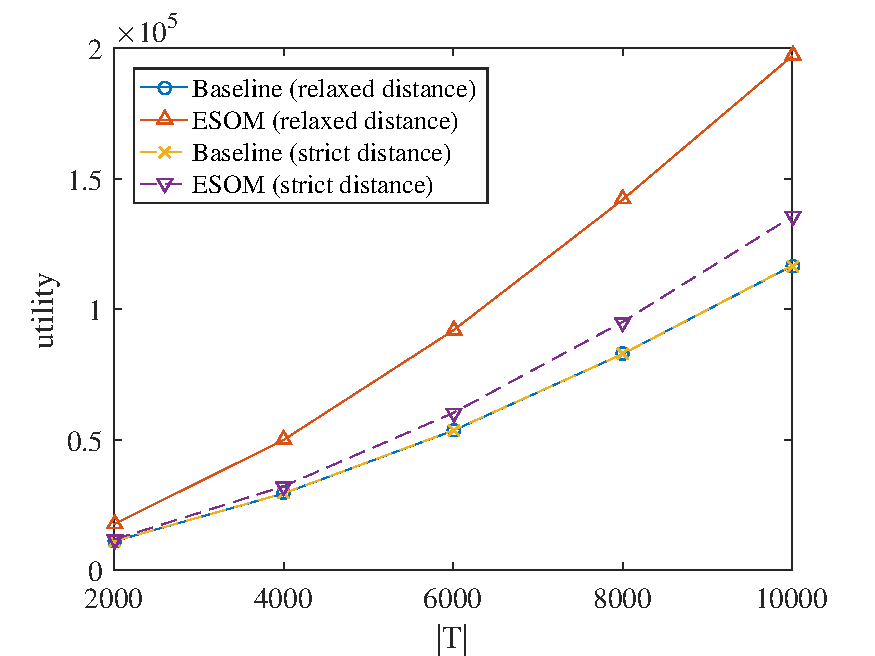
\includegraphics[height=0.16\textheight,width=0.31\textwidth]{FCS-20363-fig1.pdf}
		\label{fig:subfig:a} %% label for first subfigure	
		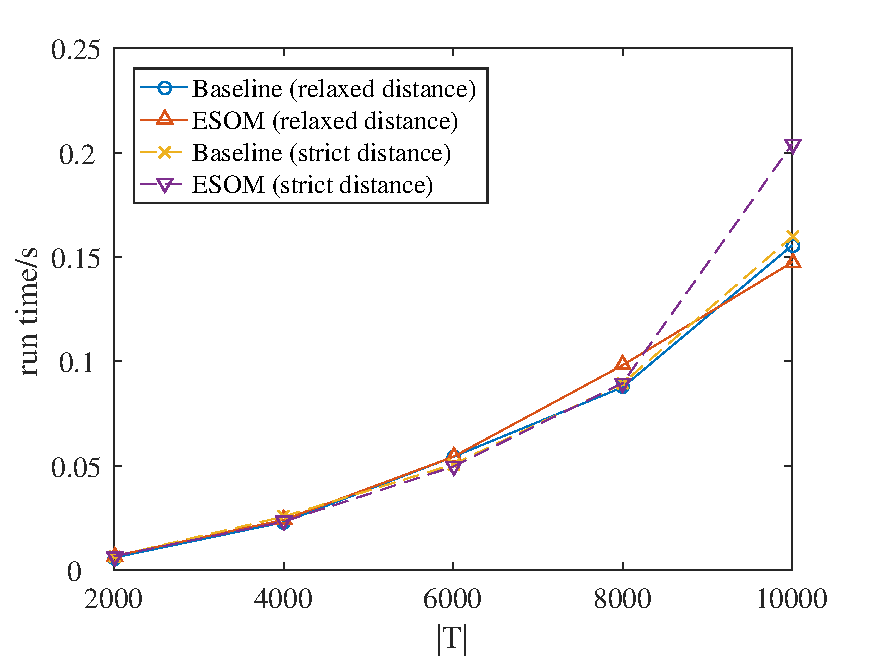
\includegraphics[height=0.16\textheight,width=0.31\textwidth]{FCS-20363-fig2.pdf}
		\label{fig:subfig:a} %% label for first subfigure	
		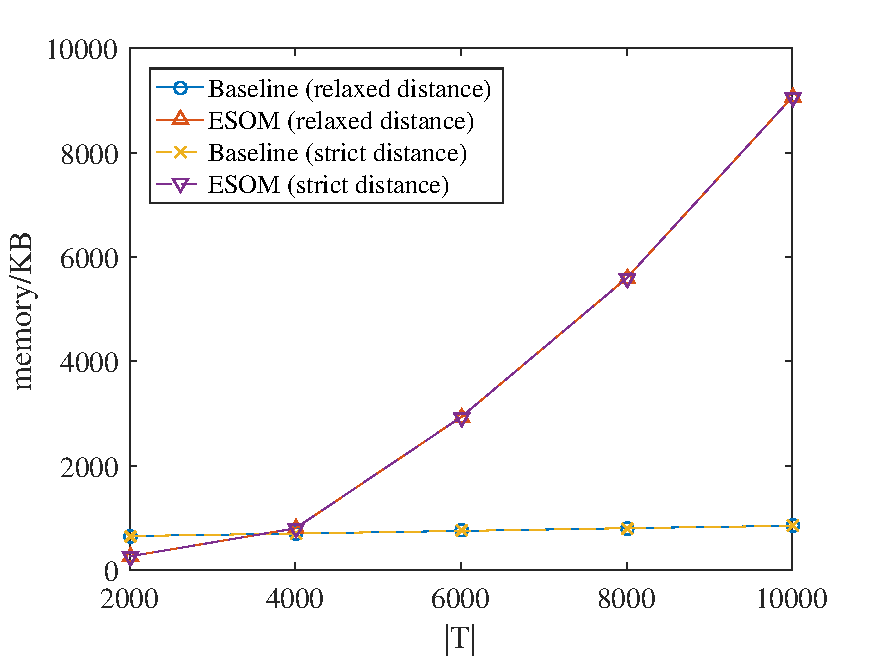
\includegraphics[height=0.16\textheight,width=0.31\textwidth]{FCS-20363-fig3.pdf}}
	\hspace{1in}
	~~	
	\caption{Results on varying $|T|$}
	\label{fig:subfig} %% label for entire figure
\end{figure*}

\textbf{Complexity Analysis}. For each time window, the time complexity of the ESOM algorithm is $O(|T_i||W_i|)$. With given $T$ and $W$ for the whole time period, the time complexity is $O(|T||W|)$.

\subsection{Competitive Ratio}

In the RMOSM problem, we simplify the competitive ratio as $\frac{M}{M^{*}}$, where $M$ is the result of the ESOM algorithm, and $M^{*}$ is the optimal result. 

\noindent \textbf{Theorem}. {\it For each time window, the profit R resulted from the ESOM algorithm satisfies that $R \geq \frac{2}{3}R^*$, where $R$ is the optimal profit.}

As in ESOM algorithm tasks with higher prices have priority to be matched, the competitive ratio of ESOM is $\frac{2}{3}$.

\section{Experimental Study}
\setcounter{subsection}{0}
\subsection{Experimental Setup}

We use one real dataset, the New York City Taxi and Limousine Commission(NYC TLC) data set\cite{NYCTLC}. We also use synthetic datasets for evaluation. We generate the location, utility and appearing time following uniform distribution, too. Statistics of the synthetic datasets are shown in Table 2.

\doublerulesep 0.1pt
\begin{table}[h]
	\begin{footnotesize}
		\caption{Synthetic Dataset}
		\label{tab:1}
		\begin{tabular}{p{2cm}p{6cm}}
			\hline\hline\noalign{\smallskip}
			Factor & \makecell[c]{Setting} \\ 
			\noalign{\smallskip}
			\hline
			$|T|$ & \makecell[c]{1000, 2000, \textbf{3000}, 4000, 5000} \\ 
			$|W|$ & \makecell[c]{1000, 2000, \textbf{3000}, 4000, 5000} \\  
			$|T|\, (|T|=|W|)$ & \makecell[c]{2000, 4000, 6000, 8000, 10000} \\
			Threshold & \makecell[c]{50, 100, \textbf{200}, 300, 400} \\
			RelaxedDistance & \makecell[c]{1, 50, \textbf{100}, 150, 180} \\
			NumberOfTimePeriods & \makecell[c]{\textbf{50}} \\
			Bound & \makecell[c]{\textbf{3000}} \\
			\hline\hline
		\end{tabular}
	\end{footnotesize}
\end{table}

\subsection{Experiment Result}
The experiment results on the synthetic datasets are shown in Fig.1.

\section{Performance Analysis}

In terms of total utility scores, the ESOM algorithm with relaxed distance always performs the best among four algorithms in both synthetic and real dataset. As for running time, with capacity's increment, the four algorithms are difference regarding to the number of matched pairs. And in the aspect of memory cost, although ESOM performs worst for the need of substitutable marks, it's efficient enough to be applied to real-time assignments with low memory cost.

\section{Conclusion}

We identify a problem about dynamic task assignment, called RMOSM Problem, then introduce the concept Substitutable and design a novel algorithm Equation-Substitutable Online Matching (ESOM). Finally we conduct experiments that verify the efficiency and effectiveness of the proposed approaches.

\bibliographystyle{unsrt}
\bibliography{ref}

\end{document}
